\BourbakiExercisesSection

\begin{enumerate}
\def\labelenumi{\arabic{enumi}.}
\item
  设 E, F 为两个 A-模，且 \(u: \mathbf{E} \to \mathbf{F}\) 为线性映射。设 M 为 E 的子模，N 为 F 的子模， \(i: \mathbf{M} \to \mathbf{E}\) 为典范单射， \(q: \mathbf{F} \to \mathbf{F} / \mathbf{N}\) 为典范满射。证明 \(u(\mathbf{M}) = \operatorname{Im}(u \circ i)\) 和 \(u^{-1}(\mathbf{N}) = \operatorname{Ker}(q \circ u)\) .
\item
  设 E 为左 A-模；对于 A 的每个左理想 a，令 aE 表示所有 ax 的和，其中 \(x \in E\) ，因此它是 E 的子模。
\end{enumerate}

\begin{enumerate}
\def\labelenumi{(\alph{enumi})}
\item
  证明对于每个 A-模族 \((\mathbf{E}_{\lambda})_{\lambda \in L}\) ，a. \(\bigoplus_{\lambda \in L} \mathbf{E}_{\lambda}\) 典范地等同于 \(\bigoplus_{\lambda \in L} a E_{\lambda}\) .
\item
  若 \(\mathfrak{a}\) 是 \(\mathbf{A}\) 的有限生成左理想，证明对每个族 \((\mathbf{E}_{\lambda})_{\lambda \in L}\) （由 \(\mathbf{A}\) -模组成）， \(\mathfrak{a}\) . \(\prod_{\lambda \in L} \mathbf{E}_{\lambda}\) 典范地等同于 \(\prod_{\lambda \in L} \mathfrak{a}\mathbf{E}_{\lambda}\) 。给出一个例子，其中 \(\mathfrak{a}\) 不是有限生成的且上述性质不成立（取 \(\mathbf{A}\) 交换且所有 \(\mathbf{E}_{\lambda}\) 都等于 \(\mathbf{A}\) ）.
\end{enumerate}

*(c) 设 K 是一个交换域，A 是 K 上两个未定元的多项式环 K{[}X,Y{]} ，m = AX 且 n = AY。若 E 是 \(\mathbf{A}^2\) 关于 \(\mathbf{A}^2\) 中由 \(\mathbf{Xe}_1 - \mathbf{Ye}_2\) 生成的子模的商 A-模 (其中 \((e_1, e_2)\) 是 \(\mathbf{A}^2\) 的典范基 )，证明 \((m \cap n)E \neq (mE) \cap (nE)\) .*

\begin{enumerate}
\def\labelenumi{\arabic{enumi}.}
\setcounter{enumi}{2}
\tightlist
\item
  设 E 是一个 A-模。
\end{enumerate}

\begin{enumerate}
\def\labelenumi{(\alph{enumi})}
\tightlist
\item
  设 \((\mathbf{L}_{\mu})_{\mu \in \mathbf{M}}\) 是一族右有向有序集，且对所有 \(\mu \in \mathbf{M}\) ，设 \((\mathrm{F}_{\lambda \mu})_{\lambda \in L_{\mu}}\) 是 \(\mathbf{E}\) 的一族递增的子模。证明
\end{enumerate}

\[
\bigcap_ {\mu \in \mathbf {M}} \left(\sum_ {\lambda \in L _ {\mu}} F _ {\lambda \mu}\right) = \sum_ {\rho \in \prod_ {\mu} L _ {\mu}} \left(\bigcap_ {\mu \in \mathbf {M}} F _ {\rho (\mu), \mu}\right).
\]

\begin{enumerate}
\def\labelenumi{(\alph{enumi})}
\setcounter{enumi}{1}
\tightlist
\item
  设 A 为一个域，E 为 A-模 \(A^{N}\) ；设 G 为 E 的子模 \(\mathbf{A}^{(\mathbf{N})}\) ；另一方面，对 N 的每个有限子集 H，设 \(F_{H}\) 为子模 \(\prod_{n\in \mathbf{N}}\mathbf{M}_n\) （ \(\mathbf{E}\) 的），其中 \(\mathbf{M}_n = \mathbf{A}\) （对于 \(n\notin \mathrm{H}\) ）且 \(\mathbf{M}_n = 0\) （对于 \(n\in \mathrm{H}\) ）。证明族 \((\mathrm{F_H})\) （其中 \(\mathbf{H}\) 遍历集 \(\Phi\) ，由 \(\mathbf{N}\) 的有限子集组成）是右有向的，并且
\end{enumerate}

\[
\left(\bigcap_ {\mathrm{H} \in \Phi} \mathrm{F} _ {\mathrm{H}}\right) + \mathrm{G} \neq \bigcap_ {\mathrm{H} \in \Phi} (\mathrm{F} _ {\mathrm{H}} + \mathrm{G}).
\]

\begin{enumerate}
\def\labelenumi{\arabic{enumi}.}
\setcounter{enumi}{3}
\tightlist
\item
  设 \(\mathbf{E}, \mathbf{F}_1, \mathbf{F}_2\) 为三个 A-模， \(f_1: \mathbf{F}_1 \to \mathbf{E}\) , \(f_2: \mathbf{F}_2 \to \mathbf{E}\) 为两个 A-线性映射。 \(\mathbf{F}_1\) 和 \(\mathbf{F}_2\) 相对于 \(f_1\) 和 \(f_2\) 的纤维积是积 \(\mathbf{F}_1 \times \mathbf{F}_2\) 中由有序对 \((x_1, x_2)\) （满足 \(f_1(x_1) = f_2(x_2)\) ）组成的子模；记作 \(\mathbf{F}_1 \times_{\mathbf{E}} \mathbf{F}_2\) .
\end{enumerate}

\begin{enumerate}
\def\labelenumi{(\alph{enumi})}
\item
  对于每一对 A-线性映射 \(u_1 \colon G \to F_1, u_2 \colon G \to F_2\) （满足 \(f_1 \circ u_1 = f_2 \circ u_2\) ），存在且仅存在一个 A-线性映射 \(u \colon G \to F_1 \times_E F_2\) ，使得 \(p_1 \circ u = u_1, p_2 \circ u = u_2\) ，其中 \(p_1\) 和 \(p_2\) 表示 \(F_1 \times_E F_2\) 上投影 \(pr_1\) 和 \(pr_2\) 的限制.
\item
  设 \(\mathbf{E}'\) , \(\mathbf{F}_1'\) , \(\mathbf{F}_2'\) 是三个A-模， \(f_1': \mathbf{F}_1' \to \mathbf{E}', f_2': \mathbf{F}_2' \to \mathbf{E}'\) 为两个 A-线性映射，而 \(\mathbf{F}_1' \times_{\mathbf{E}'} \mathbf{F}_2'\) 为相对于这些映射的纤维积。对于每一组 A-线性映射 \(v_1: \mathbf{F}_1 \to \mathbf{F}_1'\) , \(v_2: \mathbf{F}_2 \to \mathbf{F}_2'\) , \(w: \mathbf{E} \to \mathbf{E}'\) ，若 \(f_1' \circ v_1 = w \circ f_1, f_2' \circ v_2 = w \circ f_2\) ，设 \(v\) 是 \(\mathbf{F}_1 \times_{\mathbf{E}} \mathbf{F}_2\) 到 \(\mathbf{F}_1' \times_{\mathbf{E}'} \mathbf{F}_2'\) 的A-线性映射，对应于两个线性映射 \(v_1 \circ p_1\) 和 \(v_2 \circ p_2\) 。证明如果 \(v_1\) 和 \(v_2\) 是单射，则 \(v\) 也是单射；给出一个例子，其中 \(v_1\) 和 \(v_2\) 是满射但 \(v\) 不是满射（取 \(\mathbf{E}' = \{0\}\) ）。如果 \(w\) 是单射且 \(v_1\) 和 \(v_2\) 是满射，证明 \(v\) 是满射。
\end{enumerate}

\begin{enumerate}
\def\labelenumi{\arabic{enumi}.}
\setcounter{enumi}{4}
\tightlist
\item
  设 \(\mathbf{E}, \mathbf{F}_1, \mathbf{F}_2\) 为三个 A-模， \(f_1: \mathbf{E} \to \mathbf{F}_1, f_2: \mathbf{E} \to \mathbf{F}_2\) 为两个线性映射。 \(\mathbf{F}_1\) 和 \(\mathbf{F}_2\) 相对于 \(f_1\) 和 \(f_2\) 的融合和是 \(\mathbf{F}_1 \times \mathbf{F}_2\) 关于 \(\mathbf{E}\) 在映射 \(z \mapsto (f_1(z), -f_2(z))\) 下的像所成的子模的商模；记作 \(\mathbf{F}_1 \oplus_{\mathbf{E}} \mathbf{F}_2\) .
\end{enumerate}

\begin{enumerate}
\def\labelenumi{(\alph{enumi})}
\tightlist
\item
  对于每一对 A-线性映射 \(u_{1}: \mathbf{F}_{1} \to \mathbf{G}, u_{2}: \mathbf{F}_{2} \to \mathbf{G}\) ，若 \(u_{1} \circ f_{1} = u_{2} \circ f_{2}\) ，证明存在且仅存在一个 A-线性映射 \(u: \mathbf{F}_{1} \oplus_{\mathbf{E}} \mathbf{F}_{2} \to \mathbf{G}\) ，使得 \(u \circ j_{1} = u_{1}, u \circ j_{2} = u_{2}\) ，其中 \(j_{1}\) 和 \(j_{2}\) 分别表示典范映射
\end{enumerate}

\[
\mathbf {F} _ {1} \times \mathbf {F} _ {2} \rightarrow \mathbf {F} _ {1} \oplus_ {\mathrm{E}} \mathbf {F} _ {2}
\]

与典范单射 \(\mathbf{F}_1\to \mathbf{F}_1\times \mathbf{F}_2,\mathbf{F}_2\rightarrow \mathbf{F}_1\times \mathbf{F}_2.\)

\begin{enumerate}
\def\labelenumi{(\alph{enumi})}
\setcounter{enumi}{1}
\tightlist
\item
  设 \(\mathbf{E}'\) , \(\mathbf{F}_1'\) , \(\mathbf{F}_2'\) 是三个A-模， \(f_1': \mathbf{E}' \to \mathbf{F}_1'\) , \(f_2': \mathbf{E}' \to \mathbf{F}_2'\) 为两个 A-线性映射，而 \(\mathbf{F}_1' \oplus_{\mathbf{E}'} \mathbf{F}_2'\) 为相对于这些映射的融合和。对于每一组 A-线性映射 \(v_1: \mathbf{F}_1' \to \mathbf{F}_1\) , \(v_2: \mathbf{F}_2' \to \mathbf{F}_2\) , \(w: \mathbf{E}' \to \mathbf{E}\) ，若 \(v_1 \circ f_1' = f_1 \circ w\) , \(v_2 \circ f_2' = f_2 \circ w\) ，设 \(v\) 是 \(\mathbf{F}_1' \oplus_{\mathbf{E}'} \mathbf{F}_2'\) 到 \(\mathbf{F}_1 \oplus_{\mathbf{E}} \mathbf{F}_2\) 的A-线性映射，对应于两个线性映射 \(j_1 \circ v_1\) 和 \(j_2 \circ v_2\) 。证明如果 \(v_1\) 和 \(v_2\) 是满射，那么 \(v\) 也是满射；给出一个例子，其中 \(v_1\) 和 \(v_2\) 是单射但 \(v\) 不是单射。证明如果 \(w\) 是满射且 \(v_1\) 和 \(v_2\) 是单射，则 \(v\) 是单射。
\end{enumerate}

\begin{enumerate}
\def\labelenumi{\arabic{enumi}.}
\setcounter{enumi}{5}
\tightlist
\item
  给定一个 A-模 E，设 \(\gamma(E)\) 表示 E 的生成系的基数中的最小者。
\end{enumerate}

\begin{enumerate}
\def\labelenumi{(\alph{enumi})}
\tightlist
\item
  若 \(0 \to \mathbf{E} \to \mathbf{F} \to \mathbf{G} \to 0\) 是 A-模的正合序列，则
\end{enumerate}

\[
\gamma (\mathbf {G}) \leqslant \gamma (\mathbf {F}) \leqslant \gamma (\mathbf {E}) + \gamma (\mathbf {G}).
\]

给出一个乘积 \(\mathbf{F} = \mathbf{E} \times \mathbf{G}\) 的例子，使得 \(\gamma(\mathbf{E}) = \gamma(\mathbf{F}) = \gamma(\mathbf{G}) = 1\) （取 \(\mathbf{E}\) 和 \(\mathbf{G}\) 为 \(\mathbf{Z}\) 的商模 ）.

\begin{enumerate}
\def\labelenumi{(\alph{enumi})}
\setcounter{enumi}{1}
\item
  若 \(\mathbf{E}\) 是子模族 \((\mathrm{F}_{\lambda})_{\lambda \in L}\) 的和，则 \(\gamma (\mathbf{E})\leqslant \sum_{\lambda \in L}\gamma (\mathbf{F}_{\lambda}).\)
\item
  若 \(\mathbf{M}\) 和 \(\mathbf{N}\) 是模 \(\mathbf{E}\) 的子模，证明
\end{enumerate}

\[
\sup (\gamma (\mathbf {M}), \gamma (\mathbf {N})) \leqslant \gamma (\mathbf {M} \cap \mathbf {N}) + \gamma (\mathbf {M} + \mathbf {N}).
\]

\begin{enumerate}
\def\labelenumi{\arabic{enumi}.}
\setcounter{enumi}{6}
\tightlist
\item
  \begin{enumerate}
  \def\labelenumii{(\alph{enumii})}
  \tightlist
  \item
    设 A 为一个环，E 为一个 (A, A)-双模；在积 \(B = A \times E\) 上，通过令下式成立来定义环结构
  \end{enumerate}
\end{enumerate}

\[
(a, x) (a ^ {\prime}, x ^ {\prime}) = (a a ^ {\prime}, a x ^ {\prime} + x a ^ {\prime});
\]

E（典范地等同于 \(\{0\} \times \mathbf{E}\) ）于是是B的一个双边理想，使得 \(\mathbf{E}^2 = \{0\}\) .

\begin{enumerate}
\def\labelenumi{(\alph{enumi})}
\setcounter{enumi}{1}
\tightlist
\item
  通过适当选取 A 和 E，证明 E 可以是一个左 B-模，其 \(\gamma(\mathbf{E})\) （习题6）为任意基数，尽管 \(\gamma(\mathbf{B}_{s}) = 1\) .
\end{enumerate}

*8. 设 A 是一个交换环， \(\mathbf{B} = \mathbf{A}[\mathbf{X}_n]_{n\geqslant 1}\) 是 A 上含无穷多个未定元的多项式环，C 是 B 关于由多项式 \((\mathbf{X}_1 - \mathbf{X}_2)\mathbf{X}_i\) （对于 \(i\geqslant 3\) ）生成的理想的商环。若 \(\xi_1\) 和 \(\xi_2\) 分别是 \(\mathbf{X}_1\) 和 \(\mathbf{X}_2\) 在 C 中的类，证明单生成理想 \(\mathrm{C}\xi_1\) 和 \(\mathrm{C}\xi_2\) 在 C 中的交不是有限生成的理想。*

\begin{enumerate}
\def\labelenumi{\arabic{enumi}.}
\setcounter{enumi}{8}
\item
  证明：在 A-模 E 中，若 \((\mathrm{F}_{n})_{n\geqslant1}\) 是有限生成子模的一个严格递增序列，则以诸 \(F_{n}\) 之并为 E 的子模的 F 不是有限生成的。由此推出，如果 E 是一个非有限生成的 A-模，则存在 E 的一个子模 F，使得 \(\gamma(\mathrm{F})=\aleph_{0}(=\mathrm{Card}(\mathbf{N}))\) .
\item
  设 E 是一个 Z-模，它是两个子模 M、N 的直和，且分别同构于 Z/2Z 和 Z/3Z；证明：不存在将 E 分解为两个非零子模的直和的其他分解方式。
\item
  设 A 是具有左分式域 (I, § 9, 习题 15) 的环。证明在 A-模 \(A_{s}\) 中，异于 \(A_{s}\) 和 \(\{0\}\) 的子模没有互补子模（参见 I，§ 9，习题 16）。
\item
  设 \(\mathbf{G}\) 为一个模，且 \(\mathbf{E}, \mathbf{F}\) 为两个子模，使得 \(\mathbf{E} \subset \mathbf{F}\) .
\end{enumerate}

\begin{enumerate}
\def\labelenumi{(\alph{enumi})}
\item
  若 F 是 G 的直因子，则 F/E 是 G/E 的直因子。若同时 E 是 F 的直因子，则 E 是 G 的直因子。
\item
  若E是G的一个直因子，则E也是F的一个直因子。若进一步F/E是G/E的一个直因子，则F是G的一个直因子。
\item
  给出两个子模 \(\mathbf{M}, \mathbf{N}\) （ \(\mathbf{Z}\) -模 \(\mathbf{E} = \mathbf{Z}^2\) 的）的例子，使得 \(\mathbf{M}\) 和 \(\mathbf{N}\) 都是 \(\mathbf{E}\) 的直因子，但 \(\mathbf{M} + \mathbf{N}\) 不是 \(\mathbf{E}\) 的直因子.
\item
  设 \(p\) 是一个素数， \(U_p\) 是 \(\mathbf{Z}\) -模 \(\mathbf{Q} / \mathbf{Z}\) 的子模，由模 \(\mathbf{Z}\) 的类（对应于形如 \(k / p^n\) 的有理数）组成 ( \(k \in \mathbf{Z}\) , \(n \in \mathbf{N}\) )。设 \(E\) 为积 \(\mathbf{Z}\) -模 \(M \times N\) ，其中 \(M\) 和 \(N\) 都同构于 \(U_p\) ，且 \(M\) 和 \(N\) 被典范地等同于 \(E\) 的子模。考虑自同态 \(u: (x, y) \mapsto (x, y + px)\) （ \(E\) 的）；证明 \(u\) 是双射。若 \(M' = u(M)\) ，证明 \(M\) 和 \(M'\) 都是 \(E\) 的直因子，但 \(M \cap M'\) 不是 \(E\) 的直因子（利用 (b)，并证明 \(Z\) -模 \(U_p\) 除自身和 \{0\} 外没有其他直因子）.
\end{enumerate}

¶ 13. 设 E 是一个 A-模，B 为环 End\_A E。证明对于元素 \(u \in B\) ，以下三个条件等价：（1）Bu 是左 B-模 B\_s 的一个直因子；（2）uB 是右 B-模 B\_d 的一个直因子；（3）Ker(u) 和 Im(u) 是 A-模 E 的直因子。（注意，作为 B\_s 的直因子的每个左理想都具有 Bp 的形式，其中 p 是 E 中的一个投影算子；参见 I，§ 8，习题 12，并利用 II，§ 1，第 9 号，命题 15 的推论 1 和 2。）

\begin{enumerate}
\def\labelenumi{\arabic{enumi}.}
\setcounter{enumi}{13}
\tightlist
\item
  设 L 是一个良序集，E 是一个 A-模，且 \((\mathbf{E}_{\lambda})_{\lambda \in L}\) 是 E 的子模的一个递增族，使得：（1）存在 \(\lambda \in L\) 使得 \(E_{\lambda} = \{0\}\) ； (2) E 是诸 \(E_{\lambda}\) （ \(\lambda \in L\) ）的并； (3) 如果 \(\lambda \in L\) 使得 \(\mu < \lambda\) 的集合具有最大元 \(\lambda'\) , \(E_{\lambda}\) 是 \(E_{\lambda'}\) 与一个子模 \(F_{\lambda}\) 的直和；（4）若 \(\lambda \in L\) 是 \(\mu < \lambda\) 的集合的上确界，则 \(E_{\lambda}\) 是诸 \(E_{\mu}\) （ \(\mu < \lambda\) ）的并。在这些条件下，证明 E 是诸 \(F_{\lambda}\) 的直和。（用超限归纳法证明每个 \(E_{\lambda}\) 是诸 \(F_{\mu}\) 的直和，其中 \(\mu \leqslant \lambda\) 。)
\end{enumerate}

¶ 15. 设 c 为无限基数。

\begin{enumerate}
\def\labelenumi{(\alph{enumi})}
\item
  设 I 为一个集合， \(R\{a, b\}\) 为 I 的元素之间的一种关系，使得对所有 \(\alpha \in I\) ，由 \(\beta \in I\) 中使 \(R\{\alpha, \beta\}\) 成立者组成的集合具有基数 \(\leqslant c\) 。证明存在一个良序集 L 和 I 的子集的一个递增族 \((\mathrm{I}_{\lambda})_{\lambda \in L}\) ，使得：(1) 存在 \(\lambda \in L\) 使得 \(I_{\lambda} = \varnothing\) ；(2) I 是诸 \(I_{\lambda}\) （ \(\lambda \in L\) ）的并； (3) 如果 \(\lambda \in L\) 使得 \(\mu < \lambda\) 的集合有最大元 \(\lambda'\) , \(\text{Card}(\mathbf{I}_{\lambda} - \mathbf{I}_{\lambda'}) \leqslant c\) ；（4）若 \(\lambda \in L\) 是 \(\mu < \lambda\) 的集合的上确界，则 \(I_{\lambda}\) 是诸 \(I_{\mu}\) （ \(\mu < \lambda\) ）的并；(5) 若 \(\alpha \in I_{\lambda}\) 且 \(R\{\alpha, \beta\}\) 成立，则 \(\beta \in I_{\lambda}\) 。（首先注意，对所有 \(\alpha \in I\) ，由满足如下条件的 \(\beta \in I\) 组成的集合——存在一个整数 n 和一个由 I 的元素组成的序列 \((\gamma_{j})_{1 \leqslant j \leqslant n}\) ，使得 \(\gamma_{1} = \alpha, \gamma_{n} = \beta\) 且 \(R\{\gamma_{j}, \gamma_{j+1}\}\) 对 \(1 \leqslant j \leqslant n - 1\) 成立——具有基数 \(\leqslant c\) 。然后通过超限归纳法构造诸 \(I_{\lambda}\) 。）
\item
  设 E 是一个 A-模，它是子模族 \((\mathbf{M}_{\alpha})_{\alpha\in I}\) 的直和，使得 \(\gamma(\mathbf{M}_{\alpha})\leqslant c\) 对所有 \(\alpha\in I\) 成立（参见习题 6）。设 f 是 E 的一个自同态。证明存在一个良序集 L 和 I 的子集的一个递增族 \((\mathbf{I}_{\lambda})_{\lambda\in L}\) ，满足 (a) 中的性质 (1)、(2)、(3) 和 (4)，并且此外，若记 \(\mathbf{E}_{\lambda} = \bigoplus_{\alpha \in \mathbf{I}_{\lambda}} \mathbf{M}_{\alpha}\) ，则 \(f(\mathbf{E}_{\lambda}) \subset \mathbf{E}_{\lambda}\) 。（将 (a) 应用于关系 \(R\{\alpha, \beta\}\) ：“存在 \(x \in \mathbf{M}_{\alpha}\) 使得 \(f(x)\) 在 \(\mathbf{M}_{\beta}\) 中的分量 \(\neq 0\)”。）对所有满足下列条件的 \(\lambda \in \mathbf{L}\) ：\(\mu < \lambda\) 的集合有最大元 \(\lambda'\) ，记 \(\mathbf{F}_{\lambda} = \bigoplus_{\alpha \in \mathbf{I}_{\lambda} - \mathbf{I}_{\lambda'}} \mathbf{M}_{\alpha}\) 。证明 \(\mathbf{E}\) 是诸 \(\mathbf{F}_{\lambda}\) 的直和（应用习题 14）。
\item
  在 (b) 的假设和记号下，进一步假设 \(f\) 是一个投影算子，并记 \(\mathbf{P} = f(\mathbf{E})\) 。设 \(\mathbf{P}_{\lambda} = \mathbf{P} \cap \mathbf{E}_{\lambda}\) ；证明如果 \(\lambda \in \mathbf{L}\) 使得 \(\mu < \lambda\) 的集合有最大元 \(\lambda'\) , \(\mathbf{P}_{\lambda'}\) 是 \(\mathbf{P}_{\lambda}\) 的一个直因子（参见习题 12）， \(\mathbf{P}_{\lambda}'\) 作为 \(\mathbf{P}_{\lambda'}\) 在 \(\mathbf{P}_{\lambda}\) 中的互补子模同构于 \(\mathbf{F}_{\lambda}\) 的一个直因子，且 \(\gamma(\mathbf{P}_{\lambda}') \leqslant c\) 。证明 \(\mathbf{P}\) 是诸 \(\mathbf{P}_{\lambda}'\) 的直和（应用习题 14）。
\item
  由 (c) 推出，若一个 A-模 E 是子模族 \((\mathrm{M}_{\alpha})_{\alpha\in I}\) 的直和，使得 \(\gamma(\mathrm{M}_{\alpha})\leqslant\mathfrak{c}\) ，那么 E 的每个直因子 P 也是子模族 \((\mathrm{N}_{\lambda})_{\lambda\in L}\) 的直和，使得 \(\gamma(\mathrm{N}_{\lambda})\leqslant\mathfrak{c}\) .
\end{enumerate}

\begin{enumerate}
\def\labelenumi{\arabic{enumi}.}
\setcounter{enumi}{15}
\tightlist
\item
  设 A 是一个环，使得存在一个 A-模 M，它有一个由 n 个元素组成的生成系，但包含一个由 \(n + 1\) 个元素组成的自由系。
\end{enumerate}

\begin{enumerate}
\def\labelenumi{(\alph{enumi})}
\item
  证明在 \(\mathbf{A}_s^n\) 中存在一个由 \(n + 1\) 个元素组成的自由系。
\item
  推断出在 M 中存在一个无限自由系（利用 (a) 通过归纳构造这样的系）。
\item
  设 C 为一个环，E 为自由 C-模 \(\mathrm{C}_{s}^{(\mathrm{N})}, (e_{n})\) 及其典范基，A 为 E 的自同态环。设 \(u_{1}\) 和 \(u_{2}\) 表示由下列条件定义的 E 的自同态： \(u_{1}(e_{2n}) = e_{n}, u_{1}(e_{2n+1}) = 0, u_{2}(e_{2n+1}) = e_{n}, u_{2}(e_{2n}) = 0\) 对所有 \(n \geqslant 0\) 。证明 \(u_{1}\) 和 \(u_{2}\) 构成 A-模 \(A_{s}\) 的一组基，并推断出在 A-模 \(A_{s}\) 中存在无限自由系。
\end{enumerate}

*(d) 设 A 是交换域上维数 \(\geqslant 2\) 的向量空间 E 的张量代数（参见 III，§ 5，第 1 号）。证明在 A-模 \(A_s\) 中存在无限自由系（注意，E 中两个线性无关的向量在 \(A_s\) 中也线性无关，并利用 \((b)\) ）。另一方面，对于每个整数 \(n > 0\) ，A-模 \(A_s^n\) 的每个基都有 \(n\) 个元素（参见 § 7，第 2 号，命题 3）。*

\begin{enumerate}
\def\labelenumi{\arabic{enumi}.}
\setcounter{enumi}{16}
\tightlist
\item
  设 A 是一个环。
\end{enumerate}

\begin{enumerate}
\def\labelenumi{(\alph{enumi})}
\item
  证明如果 A-模 \(\mathbf{A}_s^n\) 不同构于任何 \(\mathbf{A}_s^m\) （对于 \(m > n\) ），那么，对所有 \(p < n\) , \(\mathbf{A}_s^p\) 不同构于任何 \(\mathbf{A}_s^q\) （对于 \(q > p\) ）.
\item
  证明如果 A-模 \(A_{s}^{n}\) 不包含由 \(n + 1\) 个元素组成的自由系，则 A-模 \(A_{s}^{p}\) 不包含由 \(p + 1\) 个元素组成的自由系（对 p \textless{} n）.
\end{enumerate}

\begin{enumerate}
\def\labelenumi{\arabic{enumi}.}
\setcounter{enumi}{17}
\tightlist
\item
  设 A 是一个环，且存在一个整数 \(p\) 具有如下性质：对于每一个族 \((a_i)_{1 \leqslant i \leqslant p}\) （由 A 的 \(p\) 个元素组成），存在一个族 \((c_i)_{1 \leqslant i \leqslant p}\) （由 A 的元素组成），其中至少有一个元素不是右零因子，使得 \(\sum_{i=1}^{p} c_i a_i = 0\) .
\end{enumerate}

\begin{enumerate}
\def\labelenumi{(\alph{enumi})}
\item
  对 \(n\) 用归纳法证明：对于每个族 \((x_{i})\) （由 \(p^n\) 个 \(A_s^n\) 的元素组成），存在一个族 \((c_j)\) （由 \(p^n\) 个 \(A\) 的元素组成），其中至少有一个不是右零因子，使得 \(\sum_{j} c_j x_j = 0\) .
\item
  由 (a) 和习题 16 推出，对所有 n \textgreater{} 0，A-模 \(A_{s}^{n}\) 不包含由 \(n + 1\) 个元素组成的自由系。
\end{enumerate}

\begin{enumerate}
\def\labelenumi{\arabic{enumi}.}
\setcounter{enumi}{18}
\tightlist
\item
  设A是一个非零环且无零因子。
\end{enumerate}

\begin{enumerate}
\def\labelenumi{(\alph{enumi})}
\item
  证明对于 \(n > 1\) ，A-模 \(\mathbf{A}_s^n\) 不是单生成的。
\item
  给定一个整数 \(n \geqslant 1\) ，对于 A-模 \(\mathbf{A}_s^n\) 不包含由 \(n + 1\) 个元素组成的自由系，必要条件是 A 具有左分式域（I，§9，习题15）；反之，若此条件满足，则 \(\mathbf{A}_s^n\) 不包含由 \(n + 1\) 个元素组成的自由系，无论整数 \(n > 0\) 如何（利用习题 17 和 18 以及 I，§9，习题 16。）
\item
  证明：若 A 的每个左理想都是单生成的，则 A 具有左分式域（利用 (a) 以及 I，§9，习题 16）。
\end{enumerate}

\begin{enumerate}
\def\labelenumi{\arabic{enumi}.}
\setcounter{enumi}{19}
\tightlist
\item
  \begin{enumerate}
  \def\labelenumii{(\alph{enumii})}
  \tightlist
  \item
    设 A 是具有左分式域 (I, § 9, 习题 15) 的环。设 E 是一个 A-模；证明：若在 E 中 \((x_{i})_{1\leqslant i\leqslant r}\) 是一个自由系，且 \(y,z\) 为两个元素，使得 \(x_{1},\ldots ,x_{r},y\) 与 \(x_{1},\ldots ,x_{r},z\) 都是相关系，那么 \(x_{2},\ldots ,x_{r},y,z\) 是一个相关系。
  \end{enumerate}
\end{enumerate}

\begin{enumerate}
\def\labelenumi{(\alph{enumi})}
\setcounter{enumi}{1}
\tightlist
\item
  设 A 为商环 Z/6Z，并设 \((e_{1}, e_{2})\) 为 \(A^{2}\) 的典范基；证明如果 \(a = 2e_{1} + 3e_{2}\) ，则 a 与 \(e_{1}\) 构成一个相关系，a 与 \(e_{2}\) 亦然，尽管 \(e_{1}\) 和 \(e_{2}\) 构成一个自由系。
\end{enumerate}

\begin{enumerate}
\def\labelenumi{\arabic{enumi}.}
\setcounter{enumi}{20}
\item
  设 A 为一个环，b、c 为 A 中两个非右零因子的元素，M 为 A-模 A/Abc，N 为 M 的子模 Ac/Abc。要使 N 成为 M 的一个直因子，当且仅当存在 A 中的两个元素 x、y，使得 \(xb + cy = 1\) 。（若 \(\varepsilon\) 是 1 在 M 中的类，证明 N 在 M 中的一个互补子空间由形如 \((1 - yc)\varepsilon\) 的元素生成，其零化子为理想 Ac。）
\item
  若一个A-模E存在一个以集合I为指标集的基，且A与I两个集合中至少有一个是无限的，证明E与 \(A \times I\) 等势.
\item
  \begin{enumerate}
  \def\labelenumii{(\alph{enumii})}
  \tightlist
  \item
    设 M、N 是 A 模 E 的两个子集，m 和 n 分别是它们的零化子；证明 M ∩ N 的零化子包含 m + n，并给出一个例子说明它不同于 m + n。
  \end{enumerate}
\end{enumerate}

\begin{enumerate}
\def\labelenumi{(\alph{enumi})}
\setcounter{enumi}{1}
\item
  在积模 \(\prod_{i} \mathbf{E}_{i}\) 中，子集 \(\mathbf{F}\) 的零化子是它的各投影的零化子的交。
\item
  在自由 A-模中，元素 \(\neq0\) 的零化子仅包含 A 中 0 的左因子；特别地，若 A 是无零因子环，则自由模的每个元素 \(\neq0\) 都是自由的。
\end{enumerate}

\begin{enumerate}
\def\labelenumi{\arabic{enumi}.}
\setcounter{enumi}{23}
\tightlist
\item
  设 E 是一个 A-模，M 和 N 是 E 的两个子模。M 到 N 的传送子，记为 N:M，是由 \(a \in A\) 中使 \(aM \subset N\) 成立者组成的集合；它是 A 的一个双边理想，等于 \(\text{Ann}((\mathbf{M} + \mathbf{N})/\mathbf{N})\) .
\end{enumerate}

\begin{enumerate}
\def\labelenumi{(\alph{enumi})}
\item
  设 A 是一个交换环，M 是一个 A-模，N 是 M 的一个子模，x 是 M 的一个元素；证明 \(N \cap Ax = (N:Ax)x\) .
\item
  设 A 是一个交换环，且 \(a, b\) 为 A 的两个理想。证明 \(a:b \supset a\) ，并且 \((a:b)/a\) 是同构于 \(\operatorname{Hom}(A/b, A/a)\) 的一个 A-模.
\end{enumerate}

\begin{enumerate}
\def\labelenumi{\arabic{enumi}.}
\setcounter{enumi}{24}
\item
  设 E, F 为两个 A-模，且 \(u: E \to F\) 为一个线性映射。证明映射 \((x, y) \mapsto (x, y - u(x))\) （积模 \(E \times F\) 到自身的）是 \(E \times F\) 的一个自同构。由此推出，如果存在一个线性映射 \(v: F \to E\) 和一个 \(a \in E\) ，使得 \(v(u(a)) = a\) ，则存在 \(E \times F\) 的一个自同构 w，使得 \(w(a, 0) = (0, u(a))\) .
\item
  设 E 是一个自由 A-模，其基至少包含两个元素。
\end{enumerate}

\begin{enumerate}
\def\labelenumi{(\alph{enumi})}
\item
  证明：E到自身的每一个半线性映射（相对于A的一个自同构），若它与E的所有自同构可交换，则它必为一个位似映射 \(x \mapsto \alpha x (\alpha \in \mathbf{A})\) .
\item
  由 (a) 推出， \(\operatorname{End}_{\mathbf{A}}(\mathbf{E})\) 的中心是中心位似环，同构于 A 的中心。
\item
  由 (a) 推出，群 \(\mathbf{GL}(\mathbf{E})\) 的中心是 E 的可逆中心位似的群，它同构于 A 的中心中可逆元素组成的乘法群。
\end{enumerate}

\begin{enumerate}
\def\labelenumi{\arabic{enumi}.}
\setcounter{enumi}{26}
\tightlist
\item
  设 A 是一个交换环。证明若 A 的一个理想 \(\mathfrak{J}\) 是自由 A-模，则 \(\mathfrak{J}\) 是单生成 A-模（换言之，是一个主理想）。给出一个例子，说明该命题不能推广到非交换环的左理想（习题 16）。
\end{enumerate}

\BourbakiExercisesSection

\begin{enumerate}
\def\labelenumi{\arabic{enumi}.}
\tightlist
\item
  \begin{enumerate}
  \def\labelenumii{(\alph{enumii})}
  \tightlist
  \item
    若 A 是一个无零因子的环，证明投射 A-模的每个元素 \(\neq0\) 都是自由的。
  \end{enumerate}
\end{enumerate}

\begin{enumerate}
\def\labelenumi{(\alph{enumi})}
\setcounter{enumi}{1}
\item
  给出一个投射 A-模的例子，其零化子非零（参见 I，§ 8，第 11 号）。
\item
  证明 Z-模 Q 不是投射 Z-模。*（参见《交换代数》II，§ 5，习题 11，其中给出了整环上一个有限生成但不自由的投射模的例子。）*
\end{enumerate}

\begin{enumerate}
\def\labelenumi{\arabic{enumi}.}
\setcounter{enumi}{1}
\item
  证明每个投射 A-模都是某一族投射子模的直和，其中每个投射子模都具有可数个生成元（“卡普兰斯基定理”；将 §1 的习题 15 应用于 E 是自由模的情形）。
\item
  设 \(\mathfrak{c}\) 是一个基数且 \(\mathbf{P}\) 是一个投射 A-模，使得 \(\gamma(\mathbf{P}) \leqslant \mathfrak{c}\) (§ 1,
\end{enumerate}

练习 6）。证明若 L 是具有基数为 \(\geqslant c\) 的无限基的自由 A-模，则 P ⊕ L 与 L 同构。（注意存在一个自由 A-模 M，其基的基数为 \(\leqslant c\) ，同构于 P 与一个 A-模 Q 的直和。注意 M \(^{(N)}\) 与 P ⊕ M \(^{(N)}\) 是同构的。）

¶ 4. (a) 设 E, E' 是两个 A-模，N 是 E 的一个子模，N' 是 E' 的一个子模，使得 E 是投射的且 E/N 与 E'/N' 同构。证明存在一个正合序列

\[
0 \longrightarrow \mathrm{N} \stackrel {u} {\longrightarrow} \mathrm{E} \oplus \mathrm{N} ^ {\prime} \stackrel {v} {\longrightarrow} \mathrm{E} ^ {\prime} \longrightarrow 0.
\]

（注意存在一个同态 \(f \colon \mathbf{E} \to \mathbf{E}'\) ，使得 \(f(\mathbf{N}) \subset \mathbf{N}'\) ，它在取商后给出一个同构 \(\mathbf{E} / \mathbf{N} \to \mathbf{E}' / \mathbf{N}'\) ；以与 §1 第 7 号中正合序列（29）所用方式类似的方式定义 \(u\) 和 \(v\) 。）

\begin{enumerate}
\def\labelenumi{(\alph{enumi})}
\setcounter{enumi}{1}
\item
  从（a）推出，如果 \(\mathbf{E}'\) 是投射的， \(\mathbf{E} \oplus \mathbf{N}'\) 和 \(\mathbf{E}' \oplus \mathbf{N}\) 是同构的。
\item
  设 \(0 \to \mathbf{E}_m \to \mathbf{E}_{m-1} \to \ldots \to \mathbf{E}_1 \to \mathbf{E}_0 \to 0\) 是 A-模的一个正合序列，使得 \(\mathbf{E}_0, \mathbf{E}_1, \ldots, \mathbf{E}_{m-2}\) 是投射的。证明 A-模 \(\bigoplus_{h \geqslant 0} \mathbf{E}_{m-2h}\) 和 \(\bigoplus_{h \geqslant 0} \mathbf{E}_{m-2h+1}\) 是同构的（约定： \(\mathbf{E}_i = \{0\}\) 对于 \(i < 0\) ）.
\end{enumerate}

\begin{enumerate}
\def\labelenumi{\arabic{enumi}.}
\setcounter{enumi}{4}
\item
  设 \(u\) 是从 A-模 \(\mathbf{E}\) 到 A-模 \(\mathbf{F}\) 的线性映射， \(v = {}^t u\) 为其转置。对于每个子模 \(\mathbf{N}'\) （ \(\mathbf{F}^*\) 的）， \(\mathbf{E}\) 中正交于 \(v(\mathbf{N}')\) 的子模是 \(\overline{u}^{-1}(\mathbf{N})\) ，其中 \(\mathbf{N}\) 是 \(\mathbf{F}\) 中正交于 \(\mathbf{N}'\) 的子模.
\item
  \begin{enumerate}
  \def\labelenumii{(\alph{enumii})}
  \tightlist
  \item
    若 E 是 A-模，则 E 的每个单射自同态 u 在环 \(\operatorname{End}_{\mathbf{A}}(\mathbf{E})\) 中不是左零因子。反之，若对于 E 的每个子 A-模 \(F \neq \{0\}\) 存在 E 的一个自同态 \(v \neq 0\) ，使得 \(v(\mathbf{E}) \subset \mathbf{F}\) ，则在 \(\operatorname{End}_{\mathbf{A}}(\mathbf{E})\) 中不是左零因子的元素是单射自同态。上述条件在存在线性形式 \(x' \in E^*\) 和一个 \(x \in E\) 使得 \(\langle x, x' \rangle\) 在 A 中可逆时得到满足，特别地，当 E 是自由模时得到满足。
  \end{enumerate}
\end{enumerate}

\begin{enumerate}
\def\labelenumi{(\alph{enumi})}
\setcounter{enumi}{1}
\item
  每个自同态 \(\neq 0\) （ \(\mathbf{Z}\) -模 \(\mathbf{Q}\) 的）都是双射的，尽管不存在线性形式 \(\neq 0\) 于 \(\mathbf{Q}\) 上。
\item
  设 \(U_{p}\) 为 §1 习题 12(d) 中定义的 Z-模。证明自同态 \(x \mapsto px\) （ \(U_{p}\) 的）不是单射，并且在 \(\operatorname{End}_{\mathbf{Z}}(\mathbf{U}_{p})\) 中不是左零因子。
\end{enumerate}

\begin{enumerate}
\def\labelenumi{\arabic{enumi}.}
\setcounter{enumi}{6}
\tightlist
\item
  \begin{enumerate}
  \def\labelenumii{(\alph{enumii})}
  \tightlist
  \item
    若 \(u\) 是 A-模 \(\mathbf{E}\) 的一个满射自同态，则 \(u\) 在 \(\operatorname{End}_{\mathbf{A}}(\mathbf{E})\) 中不是右零因子。反之，若对于每个子模 \(\mathbf{F} \neq \mathbf{E}\) （ \(\mathbf{E}\) 的）存在一个线性形式 \(x^{*} \in \mathbf{E}^{*}\) ，它在 \(\mathbf{F}\) 上为零且是满射的，则 \(\operatorname{End}_{\mathbf{A}}(\mathbf{E})\) 中每个不是右零因子的元素都是满射自同态。
  \end{enumerate}
\end{enumerate}

\begin{enumerate}
\def\labelenumi{(\alph{enumi})}
\setcounter{enumi}{1}
\item
  若 E 是习题 6(c) 中定义的 Z-模，证明每个自同态 \(\neq 0\) （E 的）都是满射的，尽管在 E 上不存在线性形式 \(\neq 0\) 。
\item
  证明若 E 是自由 Z-模 \(\neq0\) ，则存在 E 的非满射自同态，它们在 \(\operatorname{End}_{\mathbf{Z}}(\mathbf{E})\) 中不是右零因子。
\end{enumerate}

\begin{enumerate}
\def\labelenumi{\arabic{enumi}.}
\setcounter{enumi}{7}
\tightlist
\item
  \begin{enumerate}
  \def\labelenumii{(\alph{enumii})}
  \tightlist
  \item
    设 E 是自由 A-模，F、G 是两个 A-模，且 \(u: \mathbf{E} \to \mathbf{G}\) , \(v: \mathbf{F} \to \mathbf{G}\) 为两个线性映射。证明若 \(u(\mathbf{E}) \subset v(\mathbf{F})\) ，则存在一个线性映射 \(w: \mathbf{E} \to \mathbf{F}\) ，使得 \(u = v \circ w\) 。
  \end{enumerate}
\end{enumerate}

\begin{enumerate}
\def\labelenumi{(\alph{enumi})}
\setcounter{enumi}{1}
\item
  给出两个非零自同态 \(u, v\) （ \(\mathbf{Z}\) -模 \(\mathbf{E}\) 的，该模定义于习题 6(c)）的例子，使得不存在自同态 \(w\) （ \(\mathbf{E}\) 的）满足 \(u = v \circ w\) （尽管 \(u(\mathbf{E}) = v(\mathbf{E}) = \mathbf{E}\) ）。
\item
  给出两个自同态 \(u, v\) （ \(\mathbf{Z}\) -模 \(\mathbf{Z}\) 的）的例子，使得 \(u^{-1}(0) = v^{-1}(0) = \{0\}\) ，但不存在自同态 \(w\) （ \(\mathbf{Z}\) 的）满足 \(u = w \circ v\) （参见 §7，习题 14）。
\end{enumerate}

\begin{enumerate}
\def\labelenumi{\arabic{enumi}.}
\setcounter{enumi}{8}
\tightlist
\item
  给定一个 A-模 E，对于 E 的每个子模 M（相应地，E* 的每个子模 M'），令 M°（相应地，M'°）表示 M 在 E* 中的正交补（相应地，M' 在 E 中的正交补）。考虑以下四个性质：
\end{enumerate}

\begin{enumerate}
\def\labelenumi{(\Alph{enumi})}
\item
  典范同态 \(c_{\mathbf{E}}: \mathbf{E} \to \mathbf{E}^{**}\) 是双射。
\item
  对于 E 的每个子模 M，典范同态 \(E^{*}/M^{\circ} \rightarrow M^{*}\) 是双射。
\item
  对于 E 的每个子模 M， \(M^{\circ\circ} = M\) .
\item
  对于 E 的每一对有序子模 M、N，
\end{enumerate}

\[
(\mathbf {M} \cap \mathbf {N}) ^ {\circ} = \mathbf {M} ^ {\circ} + \mathbf {N} ^ {\circ}.
\]

\begin{enumerate}
\def\labelenumi{(\alph{enumi})}
\item
  证明条件 (B) 蕴含 (D)（证明对于 \(x^{*} \in (\mathbf{M} \cap \mathbf{N})^{\circ}\) ，存在 \(y^{*} \in \mathbf{E}^{*}\) ，使得 \(\langle x + y, y^{*} \rangle = \langle x, x^{*} \rangle\) 对于 \(x \in \mathbf{M}\) 和 \(y \in \mathbf{N}\) 成立）。
\item
  设 A 是一个无零因子的环，但不具有左分式域 \(*\) （例如，一个维数 \textgreater1 的向量空间的张量代数，参见 III，§5，习题 5） \(^{*}\) 。若取 \(E = A_{s}\) ，则条件 (A) 成立，但条件 (B)、(C)、(D) 均不成立（关于 (B)、(C)、(D) 成立而 (A) 不成立的例子，参见 §7，第 5 号，定理 6）。
\item
  取 A 为乘积环 \(\mathbf{K}^{\mathrm{I}}\) ，其中 \(\mathbf{K}\) 是一个交换域，且 I 是无限集。证明 A-模 \(\mathbf{E} = \mathbf{A}\) 满足条件 (A) 和 (B)，但不满足 (C)（注意， \(\mathbf{A}\) 的理想的零化子都具有 \(\mathbf{K}^{\mathrm{J}}\) 的形式，其中 \(\mathbf{J} \subset \mathbf{I}\) ）。
\item
  假设对于两个子模 \(\mathbf{M},\mathbf{N}\) （ \(\mathbf{E}\) 的），满足 \(\mathbf{N} \subset \mathbf{M}\) 和 \(\mathbf{N} \neq \mathbf{M}\) ，对偶 \((\mathbf{M} / \mathbf{N})^*\) 非零；证明条件 (B) 蕴含 (C)。
\item
  \(c_{\mathbf{E}}\) 的核是正交 \((\mathbf{E}^{*})^{\circ}\) （ \(\mathbf{E}^{*}\) 在 \(\mathbf{E}\) 中的）。给出一个例子，其中 \(\mathbf{E}^{*}\) 与 \((\mathbf{E}^{*})^{\circ}\) 都不为 0（考虑一个模，它包含一个元素，该元素的零化子含有一个非零因子的元素）。
\item
  设 \(\mathbf{M}\) 是 \(\mathbf{E}\) 的一个直因子；证明 \(\mathbf{M}^{\circ \circ} = \mathbf{M} + (\mathbf{E}^{*})^{\circ}\) 。
\end{enumerate}

\begin{enumerate}
\def\labelenumi{\arabic{enumi}.}
\setcounter{enumi}{9}
\tightlist
\item
  给出一个 A-线性映射 \(u: \mathbf{E} \to \mathbf{F}\) 的例子，使得 \(^t u\) 是双射但 \(u\) 既不是单射也不是满射（参见习题 6(b) 和 (c)）。
\end{enumerate}

推导出一个例子，其中 \(y_{0} \in F\) 正交于 \(^{t}u\) 的核，但方程 \(u(x) = y_{0}\) 无解。

¶ 11. 设 A 是一个环，I 是一个 A-模。I 称为内射的，如果对每个由 A-线性映射组成的正合序列 \(\mathrm{E}' \to \mathrm{E} \to \mathrm{E}''\) ，序列

\[
\operatorname{Hom} \left(\mathrm{E} ^ {\prime \prime}, \mathrm{I}\right)\rightarrow \operatorname{Hom} (\mathrm{E}, \mathrm{I}) \rightarrow \operatorname{Hom} \left(\mathrm{E} ^ {\prime}, \mathrm{I}\right)
\]

是正合的。

\begin{enumerate}
\def\labelenumi{(\alph{enumi})}
\tightlist
\item
  证明以下性质是等价的：
\end{enumerate}

\((\alpha)\) I 是单射。

(β) 对每个由 A-线性映射组成的正合序列 \(0 \rightarrow E' \rightarrow E \rightarrow E'' \rightarrow 0\) ，序列

\[
0 \rightarrow \operatorname{Hom} (\mathrm{E} ^ {\prime \prime}, \mathrm{I}) \rightarrow \operatorname{Hom} (\mathrm{E}, \mathrm{I}) \rightarrow \operatorname{Hom} (\mathrm{E} ^ {\prime}, \mathrm{I}) \rightarrow 0
\]

是正合的。

(γ) 对每个 A-模 M 及 M 的每个子模 N，从 N 到 I 的每个 A-线性映射都能延拓为从 M 到 I 的 A-线性映射。

(δ) 对于 A 的每个左理想 \(\mathfrak{a}\) 以及每个 A-线性映射 \(f: \mathfrak{a} \to \mathbf{I}\) ，存在一个元素 \(b \in \mathbf{I}\) ，使得 \(f(a) = ab\) 对所有 \(a \in \mathfrak{a}\) 成立。

(ζ) I 是包含它的每个 A-模的一个直因子。

(θ) 对于每个 A-模 E，若 E 是 I 与一个单生成子模的和，则 I 是 E 的一个直因子。

为证明(δ)蕴含(γ)，需说明性质(δ)蕴含：若E是A-模，F是E的子模且E/F是单生成的，则F到I的每个线性映射都能延拓为E到I的线性映射。然后使用Zorn引理。为证明 (θ) 蕴含 (δ)，考虑 A-模 \(A_{s} \times I = M\) 以及 M 的由元素 \((a, -f(a))\) （对于 \(a \in \mathfrak{a}\) ）组成的子模 N，并将 (θ) 应用于商模 M/N。）

\begin{enumerate}
\def\labelenumi{(\alph{enumi})}
\setcounter{enumi}{1}
\tightlist
\item
  对于 Z-模 E 为内射模，其充要条件是：对所有 \(x \in E\) 以及每个整数 \(n \neq 0\) ，存在 \(y \in E\) 使得 ny = x。特别地，Z-模 Q 和 Q/Z 是内射的。
\end{enumerate}

\begin{enumerate}
\def\labelenumi{\arabic{enumi}.}
\setcounter{enumi}{11}
\tightlist
\item
  \begin{enumerate}
  \def\labelenumii{(\alph{enumii})}
  \tightlist
  \item
    A-模的一个乘积 \(\prod_{\lambda \in L} E_{\lambda}\) （习题 11）为内射的充要条件是每个 \(E_{\lambda}\) 都是内射的。
  \end{enumerate}
\end{enumerate}

\begin{enumerate}
\def\labelenumi{(\alph{enumi})}
\setcounter{enumi}{1}
\tightlist
\item
  设 K 是一个交换域，L 是一个无限集，A 是乘积环 \(K^{L}\) 。证明 A 是一个内射 A-模（利用 (a)），但 A 的理想 \(\mathfrak{a}\) —— \(K^{L}\) 的因子的直和（典范地等同于 A 的理想）——不是内射 A-模。
\end{enumerate}

¶ 13. (a) 设 A 为一个环，I 为一个内射 A-模（习题 11），使得对于每一个非零单生成 A-模 E，都存在一个从 E 到 I 的非零 A-同态。设 M 为一个 A-模，N 为 M 的一个子模，且 \(\tilde{\mathbf{N}}\) 为由 \(u \in \operatorname{Hom}_{\mathbf{A}}(\mathbf{M}, \mathbf{I})\) （满足 \(u(x) = 0\) 于 N 中）组成的集合。证明对于所有 \(y \notin N\) ，存在一个 \(u \in \tilde{\mathbf{N}}\) ，使得 \(u(y) \neq 0\) 。

\begin{enumerate}
\def\labelenumi{(\alph{enumi})}
\setcounter{enumi}{1}
\item
  设 A 为一个环。对于每个 (A, A)-双模 T 以及每个左（相应地，右）A-模 M， \(\operatorname{Hom}_{\mathbf{A}}(\mathbf{M}, \mathbf{T})\) 典范地具有一个右（相应地，左）A-模结构，它源自 T 上的模结构，并且存在一个典范 A-同态 \(c_{M,T}: M \to \operatorname{Hom}_{\mathbf{A}}(\operatorname{Hom}_{\mathbf{A}}(\mathbf{M}, \mathbf{T}), \mathbf{T})\) ，使得 \(c_{M,T}(x)\) 是 A-同态 \(u \mapsto u(x)\) 。证明：若 I 是一个 (A, A)-双模，且作为左 A-模满足 (a) 中的条件，则典范同态 \(c_{M,I}\) 对每个左 A-模 M 都是单射。
\item
  设 I 是一个 (A, A)-双模，它作为左 A-模和右 A-模都是内射的，并且对于每一个（左或右）单生成 A-模 \(E \neq 0\) ，都存在从 E 到 I 的非零 A-同态。证明在这些条件下，若 P 是左（相应地，右）投射 A-模，则 \(\operatorname{Hom}_{\mathbf{A}}(\mathbf{P}, \mathbf{I})\) 是右（相应地，左）内射 A-模。（假设 P 是左投射 A-模。注意对右 A-模 N 的每个子模 \(N'\) ， \(\operatorname{Hom}_{\mathbf{A}}(\mathbf{N}', \mathbf{I})\) 同构于 \(\operatorname{Hom}_{\mathbf{A}}(\mathbf{N}, \mathbf{I})\) 的一个商模，并将 (b) 应用于右模 N 和左模 P。）
\item
  设 C 为交换环，A 为 C-代数，I 为内射 C-模，使得对每个单生成 C-模 \(E \neq \{0\}\) 存在一个从E到I的非零C-同态。对于每个A-模M， \(\operatorname{Hom}_{\mathbf{C}}(\mathbf{M}, \mathbf{I})\) 是一个A-模；证明对于每个投射A-模P， \(\operatorname{Hom}_{\mathbf{C}}(\mathbf{P}, \mathbf{I})\) 是一个内射A-模（论证与(c)相同）。
\end{enumerate}

\begin{enumerate}
\def\labelenumi{\arabic{enumi}.}
\setcounter{enumi}{13}
\tightlist
\item
  设 A 为一个环。证明：对于每一个 A-模 M，都存在一个内射 A-模 I，使得 M 同构于 I 的一个子模。（取 C = Z，应用习题 13(d)，并利用习题 11(b) 以及每个 A-模都是某个自由 A-模的商模这一事实。）
\end{enumerate}

¶ 15. 一个 A-模同态 \(u: \mathbf{E} \to \mathbf{F}\) 称为本性的，如果它是单射的，并且对于每个子模 \(\mathbf{P} \neq \{0\}\) （ \(\mathbf{F}\) 的）， \(u^{-1}(\mathbf{P}) \neq \{0\}\) ；只需该条件对每个单生成子模 \(\mathbf{P} \neq \{0\}\) （ \(\mathbf{F}\) 的）成立即可。若 \(\mathbf{E}\) 是 \(\mathbf{F}\) 的子模，则称 \(\mathbf{F}\) 为 \(\mathbf{E}\) 的本性扩张，如果典范单射 \(\mathbf{E} \to \mathbf{F}\) 是本性的。

\begin{enumerate}
\def\labelenumi{(\alph{enumi})}
\item
  设 \(u: \mathbf{E} \to \mathbf{F}\) , \(v: \mathbf{F} \to \mathbf{G}\) 是两个 A-模的 A-同态。如果 \(u\) 和 \(v\) 都是本性的，则 \(v \circ u\) 也是本性的。反之，若 \(v \circ u\) 是本性的且 \(v\) 是单射，则 \(u\) 和 \(v\) 都是本性的。
\item
  设 E 是 A-模 F 的一个子模，并设 \((\mathbf{F}_{\lambda})_{\lambda \in L}\) 是 F 的一族子模，包含 E 且其并集为 F。证明：若每个 \(F_{\lambda}\) 都是 E 的本性扩张，则 F 也是。
\item
  设 \((u_{\lambda})_{\lambda \in L}\) 是一族本性同态 \(u_{\lambda} \colon \mathbf{E}_{\lambda} \to \mathbf{F}_{\lambda}\) 。证明同态 \(\bigoplus_{\lambda \in L} u_{\lambda} \colon \bigoplus_{\lambda \in L} \mathbf{E}_{\lambda} \to \bigoplus_{\lambda \in L} \mathbf{F}_{\lambda}\) 是本性的。（先就 \(L\) 只有两个元素的情形证明，然后使用 (b)。）
\item
  \(\mathbf{Z}\) -模 \(\mathbf{Q}\) 是 \(\mathbf{Z}\) 的一个本性扩张，但乘积 \(\mathbf{Q}^{\mathrm{N}}\) 不是 \(\mathbf{Z}^{\mathrm{N}}\) 的本性扩张。
\item
  设 E 是模 F 的一个子模。证明存在一个子模
\end{enumerate}

F 的一个子模 Q，使得 \(Q \cap E = \{0\}\) ，并且典范同态 \(F \to F/Q\) 在 E 上的限制是本性的。

\begin{enumerate}
\def\labelenumi{\arabic{enumi}.}
\setcounter{enumi}{15}
\tightlist
\item
  A-模 F 的子模 E 称为关于 F（或在 F 中）不可约的，如果 \(E \neq F\) 且 E 不是 F 的两个不同于 E 的子模的交集。
\end{enumerate}

\begin{enumerate}
\def\labelenumi{(\alph{enumi})}
\item
  A-模 F 是其每个子模 \(\neq \{0\}\) 的本性扩张的充要条件是： \(\{0\}\) 关于 F 是不可约的。
\item
  设 \((\mathbf{E}_{\lambda})_{\lambda \in L}\) 是 A-模 \(\mathbf{F}\) 的一族子模。称 \((\mathbf{E}_{\lambda})_{\lambda \in L}\) 为 \(\{0\}\) 在 \(\mathbf{F}\) 中的一个既约不可约分解，如果每个 \(\mathbf{F}_{\lambda}\) 都在 \(\mathbf{F}\) 中不可约，诸 \(\mathbf{E}_{\lambda}\) 的交集化为 0，并且没有哪个 \(\mathbf{E}_{\lambda}\) 包含诸 \(\mathbf{E}_{\mu}\) （ \(\mu \neq \lambda\) ）的交集。在此情形下，证明 \(\mathbf{F}\) 到 \(\bigoplus_{\lambda \in L} (\mathbf{F} / \mathbf{E}_{\lambda})\) 中的典范同态是本性的（若 \(\mathbf{E}_{\lambda}' = \bigcap_{\mu \neq \lambda} \mathbf{E}_{\mu}\) ，注意像 \(\mathbf{F}_{\lambda}'\) （ \(\mathbf{E}_{\lambda}'\) 在 \(\mathbf{F} / \mathbf{E}_{\lambda}\) 中的）非零，且 \(\mathbf{F}\) 在 \(\bigoplus_{\lambda \in L} (\mathbf{F} / \mathbf{E}_{\lambda})\) 中的像包含 \(\bigoplus_{\lambda \in L} \mathbf{F}_{\lambda}'\) ；然后应用习题 15(c)）。反之，若 \((\mathbf{E}_{\lambda})_{\lambda \in L}\) 是 \(\mathbf{F}\) 的子模的一个族，在 \(\mathbf{F}\) 中不可约，且典范同态 \(\mathbf{F} \to \bigoplus_{\lambda \in L} (\mathbf{F} / \mathbf{E}_{\lambda})\) 是本性的，则族 \((\mathbf{E}_{\lambda})\) 是 \(\{0\}\) 在 \(\mathbf{F}\) 中的一个既约不可约分解。
\end{enumerate}

¶ 17. (a) 设 M, N, M', N' 是模 E 的四个子模，使得 M ∩ N = M' ∩ N' = P。证明

\[
\mathbf {M} = (\mathbf {M} + (\mathbf {N} \cap \mathbf {M} ^ {\prime})) \cap (\mathbf {M} + (\mathbf {N} \cap \mathbf {N} ^ {\prime})).
\]

由此推出，如果 \(\mathbf{M}\) 在 \(\mathbf{E}\) 中不可约，则必然有 \(\mathbf{P} = \mathbf{M}' \cap \mathbf{N}\) 或 \(\mathbf{P} = \mathbf{N}' \cap \mathbf{N}\) 。

\begin{enumerate}
\def\labelenumi{(\alph{enumi})}
\setcounter{enumi}{1}
\tightlist
\item
  设 \((\mathrm{N}_{i})_{1\leqslant i\leqslant n}\) 是 E 中不可约子模的有限族，M 为其交集。证明若 \((\mathrm{P}_{j})_{1\leqslant j\leqslant m}\) 是 E 的子模的有限族，使得 \(M=\bigcap_{j}P_{j}\) ，那么对于每个满足 \(1\leqslant i\leqslant n\) 的指标 i，存在一个指标 \(\phi(i)\) ，使得 \(1\leqslant\phi(i)\leqslant m\) ，并且使得，如果我们写 \(N_{i}^{\prime}=\bigcap_{k\neq i}N_{k}\) ，则 \(M=P_{\phi(i)}\cap N_{i}^{\prime}\) （利用 (a)）。由此推出，如果没有哪个 \(P_{j}\) 包含诸 \(P_{k}\) （下标 \(\neq j\) 者）的交集，则 \(m\leqslant n\) （依次将 \(N_{i}\) 替换为合适的 \(P_{j}\) ，利用上述结果）。由此得出结论：M 在 E 中的两个既约不可约分解，若其中一个是有限的，则它们必然具有相同的项数（参见习题 23）。
\end{enumerate}

¶ 18. (a) 为使一个 A-模 I 是内射的，证明其必要且充分条件是 I 不具有任何不同于自身的本性扩张（证明此条件蕴含习题 11(a) 的条件 (δ)，论证方式与该习题中 (θ) 蕴含 (δ) 的证明相同）。

\begin{enumerate}
\def\labelenumi{(\alph{enumi})}
\setcounter{enumi}{1}
\item
  设 I 为内射 A-模。对于 I 的子模 E 而言，E 为内射模当且仅当 E 不具有任何不同于自身且包含在 I 中的本性扩张（利用习题 15(e)），证明此条件蕴含 E 是 I 的直因子）。
\item
  设 I 是内射 A-模，E 是 I 的子模，且 \(h: \mathbf{E} \to \mathbf{F}\) 是一个本性同态。证明存在一个单同态 \(j: \mathbf{F} \to \mathbf{I}\) ，使得 \(j \circ h\) 是 E 到 I 的典范单射。
\item
  设 I 为 A-模，E 为 I 的子模。证明以下性质等价：
\end{enumerate}

(α) I 是内射的，并且是 E 的一个本性扩张。

(β) I 是内射的，并且对于每个单同态 \(j\) （从 \(E\) 到一个内射 A-模 \(J\) 中的），存在一个从 \(I\) 到 \(J\) 的单同态，它扩张 \(j\) 。

(γ) I 是内射的，并且是 I 的包含 E 的最小内射子模。

(δ) I 是 E 的本性扩张，并且对于每个本性同态 \(h: E \to F\) ，存在一个单同态 \(j: F \to I\) ，使得 \(j \circ h\) 是 E 到 I 的典范单射。

（利用 (c) 和 (a)。）当这些等价条件成立时，I 称为 E 的内射包络；此时 I 也是 I 的包含 E 的每个子模的内射包络。

\begin{enumerate}
\def\labelenumi{(\alph{enumi})}
\setcounter{enumi}{4}
\item
  设 I 是内射 A-模，E 是 I 的子模。证明：包含在 I 中的 E 的本性扩张所成的集合的每个极大元都是 E 的一个内射包络（利用 (b)）。特别地，每个 A-模都具有内射包络（参见习题 14）。
\item
  若 I, I' 是同一个 A-模 E 的两个内射包络，证明存在从 I 到 I' 的同构，且该同构保持 E 的元素不变。
\end{enumerate}

¶ 19. (a) 设 E, F 是两个 A-模，M 是 E ⊕ F 的一个内射子模。设 I 是 M ∩ E 在 M 中的内射包络，J 是 I 在 M 中的互补子模。证明 E ⊕ F 到 E（相应地，F）上的典范投影在 I（相应地，J）上的限制是单射（将 M ∩ E → I 的单射的一个扩张 E → I 与 I 到 E 上的投影复合）。

\begin{enumerate}
\def\labelenumi{(\alph{enumi})}
\setcounter{enumi}{1}
\tightlist
\item
  设 E 是 A-模，M 是 E 的子模，且在 E 的内射子模集合中是极大的；M 在 E 中具有一个互补子模 N，它不包含任何内射子模 \(\neq\{0\}\) 。证明：对于 E 的每个内射子模 P，P 在 E 到 M 上的投影（在 E 的直和分解 \(M \oplus N\) 下）下的像是 \(P \cap M\) 在 M 中的一个内射包络（利用 (a)）。若 \(M'\) 是 E 的另一个子模，且在 E 的内射子模集合中是极大的，证明存在 E 的一个自同构将 M 变为 \(M'\) 并保持 N 的元素不变。
\end{enumerate}

¶ 20. (a) 设 A 是一个环，具有一个左分式域 K（I，§ 9，习题 15）。证明 K 看作左 A-模时是 A \(_{s}\) 的内射包络。（应用习题 18(d) 的判据 (α) 和习题 11(a) 的判据 (δ)，注意到若 f: a → K 是 A 的左理想 a 到 K 中的 A-线性映射，则元素 \(x^{-1}f(x)\) （对于 \(x \in \mathfrak{a}, x \neq 0\) ，逆元在 K 中取）不依赖于 \(x \in \mathfrak{a}\) 。）

\begin{enumerate}
\def\labelenumi{(\alph{enumi})}
\setcounter{enumi}{1}
\tightlist
\item
  设 \(U_{p}\) 为 Q/Z 的子 Z-模，由形如 \(k/p^{n}\) 的有理数的典范像组成，其中 p 是给定的素数， \(k \in Z\) 和 \(n \in N\) （II，§1，习题 12(d)）。证明 \(U_{p}\) 是每个 Z-模 \(p^{-n}Z/Z\) （同构于 \(Z/p^{n}Z\) 的）的内射包络。证明存在 \(U_{p}\) 的自同构，它们不同于恒等自同构，但保持某个子模 \(p^{-n}Z/Z\) 的元素不变。
\end{enumerate}

¶ 21. (a) 设 \((\mathbf{E}_j)_{j \in J}\) 是 A-模的一个有限族，且对所有 \(j \in J\) ，设 \(I_j\) 是 \(E_j\) 的一个内射包络；证明 \(\bigoplus_{j \in J} I_j\) 是 \(\bigoplus_{j \in J} E_j\) 的一个内射包络。

\begin{enumerate}
\def\labelenumi{(\alph{enumi})}
\setcounter{enumi}{1}
\tightlist
\item
  一个 A-模 M 称为不可分解的，如果它不同于 \(\{0\}\) 并且它不是两个不同于 \(\{0\}\) 的子模的直和。证明：若 I 是一个内射 A-模，则以下性质等价：
\end{enumerate}

\((\alpha)\) \(\{0\}\) 是 I 中的一个不可约子模。

(β) I 是不可分解的。

(γ) I 是其每个子模 \(\neq0\) 的内射包络。（利用 (a) 和习题 18 (e)。）

(δ) I 同构于内射包络 \(\mathrm{I}(\mathrm{A}/\mathrm{q})\) ，其中 q 是 A 的一个不可约左理想。

此外，当这种情况成立时，对 I 中所有 \(x \neq 0\) ， \(\operatorname{Ann}(x)\) 是 A 的一个不可约左理想，且 I 同构于 \(\operatorname{I}(\mathbf{A} / \operatorname{Ann}(x))\) 。

由此推出，A-模 E 的内射包络是不可分解的，其充分必要条件为 \(\{0\}\) 是 E 的一个不可约子模。

\begin{enumerate}
\def\labelenumi{(\alph{enumi})}
\setcounter{enumi}{2}
\item
  给出一个不可分解 Z-模 E 的例子，使得其内射包络 I(E) 是可分解的（参见 VII，§3，习题 5）。
\item
  设 E 是一个 A-模，I 是 E 的一个内射包络，且 \(I = \bigoplus_{\lambda \in L} I_{\lambda}\) 是 I 作为有限个不可分解内射子模的直和的一个分解；对所有 \(\lambda \in L\) ，设 \(J_{\lambda} = \bigoplus_{\mu \neq \lambda} I_{\mu}\) ，并设 \(N_{\lambda} = J_{\lambda} \cap E\) 。证明 \((\mathrm{N}_{\lambda})_{\lambda \in L}\) 是 \(\{0\}\) 在 E 中的一个既约不可约分解（习题 16 (b)），并且 \(I_{\lambda}\) 是 \(E/N_{\lambda}\) 的一个内射包络。反之， \(\{0\}\) 在 E 中的每一个既约不可约分解都可以由上述过程唯一地（在同构意义下）得到（使用习题 16 (b)）。
\end{enumerate}

\begin{enumerate}
\def\labelenumi{\arabic{enumi}.}
\setcounter{enumi}{21}
\tightlist
\item
  设 I 是一个内射 A-模。若 I 是不可分解的，则 I 的每一个单射自同态都是 I 的自同构。由此推出，I 不可分解的充分必要条件是环 End(I) 中所有不可逆元素构成该环的一个双边理想。
\end{enumerate}

¶ 23. 设 M 是一个 A-模，它是一个子模族（有限或非有限） \((\mathbf{M}_{\lambda})_{\lambda \in L}\) 的直和，使得对所有 \(\lambda \in L\) ， \(\operatorname{End}(\mathbf{M}_{\lambda})\) 的不可逆元素构成该环的一个双边理想（这意味着 \(\mathbf{M}_{\lambda}\) 是不可分解的）。

\begin{enumerate}
\def\labelenumi{(\alph{enumi})}
\item
  设 \(f, g\) 是 \(\mathbf{M}\) 的两个自同态，满足 \(f + g = 1_{\mathbf{M}}\) 。证明：对于互异指标的每个有限序列 \((\lambda_k)_{1 \leqslant k \leqslant s}\) （在 \(\mathbf{L}\) 中取的），存在一个子模族 \(\mathbf{N}_k\) ( \(1 \leqslant k \leqslant s\) )（ \(\mathbf{M}\) 的），使得对每个 \(k\) ，自同态 \(f, g\) 之一限制在 \(\mathbf{M}_{\lambda_{k}}\) 上时是该子模到 \(\mathbf{N}_k\) 上的一个同构，并且 \(\mathbf{M}\) 是诸 \(\mathbf{N}_k\) ( \(1 \leqslant k \leqslant s\) ) 与诸 \(\mathbf{M}_{\lambda}\) （ \(\lambda\) 不同于 \(\lambda_k\) 者）的直和。（化简到 \(s = 1\) 的情形；若 \(\pi_{\lambda}\) 是 \(\mathbf{M}\) 到 \(\mathbf{M}_{\lambda}\) 上的典范投影——对应于 \(\mathbf{M}_{\lambda}\) 与 \(\bigoplus_{\mu \neq \lambda} \mathbf{M}_{\mu}\) 的直和分解——注意 \(\pi_{\lambda} \circ f\) 或 \(\pi_{\lambda} \circ g\) 之一限制在 \(\mathbf{M}_{\lambda}\) 上时是 \(\mathbf{M}_{\lambda}\) 的一个自同构。）
\item
  设 \(f\) 是 \(\mathbf{M}\) 的一个幂等自同态。证明存在至少一个指标 \(\lambda \in \mathbf{L}\) ，使得 \(f\) 在 \(\mathbf{M}_{\lambda}\) 上的限制是 \(\mathbf{M}_{\lambda}\) 到 \(f(\mathbf{M}_{\lambda})\) 上的一个同构；此外 \(f(\mathbf{M}_{\lambda})\) 是 \(\mathbf{M}\) 的一个直因子。（若 \(g = 1_{\mathbf{M}} - f\) ，注意存在一个有限的指标序列 \((\lambda_k)_{1 \leqslant k \leqslant s}\) ，使得 \(\operatorname{Ker}(g)\) 与诸 \(\mathbf{M}_{\lambda_k}\) 的直和的交 \(\neq \{0\}\) ，并利用 (a)。）
\item
  从 (b) 推出，M 的每个不可分解直因子都同构于某个 \(M_{\lambda}\) 。
\item
  设 \((\mathrm{N}_{\kappa})_{\kappa\in K}\) 是 M 的一族不可分解子模，M 是它们的直和；由 (c)，每个 \(N_{\kappa}\) 同构于某个 \(M_{\lambda}\) ，反之亦然。设 T 为 M 的不可分解子模的类（在同构关系下）的集合，使得某个 \(M_{\lambda}\) （或某个 \(N_{\kappa}\) ）属于这些类之一。对所有 \(t\in T\) ，设 \(\mathrm{R}(t)\) （相应地 \(\mathrm{S}(t)\) ）为 \(\lambda\in L\) （相应地 \(\kappa\in K\) ）中使 \(M_{\lambda}\in t\) （相应地 \(N_{\kappa}\in t\) ）者组成的集合。证明：对所有 \(t\in T\) , \(\mathrm{Card}(\mathrm{R}(t))=\mathrm{Card}(\mathrm{S}(t))\) 。（在 (a) 的记号中，令 \(\mathrm{J}(\kappa)\) 为由满足如下条件的 \(\lambda\in L\) 组成的集合： \(\pi_{\lambda}\) 在 \(N_{\kappa}\) 上的限制是 \(N_{\kappa}\) 到 \(M_{\lambda}\) 上的一个同构；证明 \(\mathrm{J}(\kappa)\) 是有限的，并且诸 \(\mathrm{J}(\kappa)\) 覆盖 \(\mathrm{R}(t)\) （当 \(\kappa\) 遍历 \(\mathrm{S}(t)\) 时）。由此推出， \(\mathrm{Card}(\mathrm{S}(t))\leqslant\mathrm{Card}(\mathrm{R}(t))\) （当 \(\mathrm{R}(t)\) 无限时）。当 \(\mathrm{R}(t)\) 有限时，借助 (a) 证明 M 是诸 \(M_{\lambda}\) （ \(\lambda\notin R(t)\) ）与 \((\mathrm{N}_{\kappa})_{\kappa\in\mathrm{S}(t)}\) 的一个基数为 \(\mathrm{R}(t)\) 的子族的直和。
\item
  由 (d) 以及习题 22 和习题 21(d) 推出，若 \((\mathbf{E}_{\lambda})_{\lambda \in L}\) 和 \((\mathbf{E}_{\kappa}^{\prime})_{\kappa \in K}\) 是 \(\{0\}\) 在模 F 中的两个既约不可约分解，则 L 与 K 是等势的。
\end{enumerate}

\begin{enumerate}
\def\labelenumi{\arabic{enumi}.}
\setcounter{enumi}{23}
\item
  设 M 是一个 A-模，I 是它的内射包络（习题 18）， \(\mathfrak{a}\) 是 A 的一个双边理想，Q 为 I 的由 \(z \in I\) （满足 \(\mathfrak{a}z = \{0\}\) ）组成的子模；Q 具有一个自然的 \((\mathrm{A}/\mathfrak{a})\) -模结构。设 N 为 M 的由 \(x \in M\) （满足 \(\mathfrak{a}x = \{0\}\) ）组成的子模；若将 N 视为一个 \((\mathrm{A}/\mathfrak{a})\) -模，证明 Q 同构于 N 的一个内射包络。
\item
  \begin{enumerate}
  \def\labelenumii{(\alph{enumii})}
  \tightlist
  \item
    要使 A-模 \(\mathbf{Q}\) 是内射的，只需：对每个投射 A-模 P 及 P 的每个子模 \(P'\) ，每个从 \(P'\) 到 Q 的线性映射都能扩张为从 P 到 Q 的线性映射（利用每个 A-模都是某个投射 A-模的商模这一事实）。
  \end{enumerate}
\end{enumerate}

\begin{enumerate}
\def\labelenumi{(\alph{enumi})}
\setcounter{enumi}{1}
\tightlist
\item
  要使 A-模 P 是投射的，只需：对每个内射 A-模 Q 及 Q 的每个商模 \(Q''\) ，每个从 P 到 \(Q''\) 中的同态都具有 \(\phi \circ u\) 的形式，其中 \(\phi: Q \to Q''\) 是典范同态，而 u 是从 P 到 Q 中的同态（利用每个 A-模都是某个内射 A-模的子模这一事实）。
\end{enumerate}

\begin{enumerate}
\def\labelenumi{\arabic{enumi}.}
\setcounter{enumi}{25}
\tightlist
\item
  对于每个 Z-模 G 和每个整数 n \textgreater{} 0，令 \(_{n}G\) 表示 G 的自同态 \(x \mapsto nx\) 的核。若 \(0 \to G' \to G \to G'' \to 0\) 是正合序列，定义典范同态 \(d:_{n}G'' \to G'/nG'\) 使得序列
\end{enumerate}

\[
0 \longrightarrow_ {n} G ^ {\prime} \longrightarrow_ {n} G ^ {\prime \prime} \stackrel {d} {\longrightarrow} G ^ {\prime} / n G ^ {\prime} \longrightarrow G / n G \longrightarrow G ^ {\prime \prime} / n G ^ {\prime \prime} \longrightarrow 0
\]

正合。若 \(_n\mathrm{G}\) 和 \(\mathrm{G} / n\mathrm{G}\) 是有限的，我们记

\[
h _ {n} (\mathrm{G}) = \operatorname{Card} (\mathrm{G} / n \mathrm{G}) - \operatorname{Card} (_ {n} \mathrm{G});
\]

则证明 \(_{n}G'\) , \(_{n}G''\) , \(G'/nG'\) , \(G''/nG''\) 是有限的，并且

\[
h _ {n} (\mathrm{G}) = h _ {n} \left(\mathrm{G} ^ {\prime}\right) + h _ {n} \left(\mathrm{G} ^ {\prime \prime}\right).
\]

\BourbakiExercisesSection

\begin{enumerate}
\def\labelenumi{\arabic{enumi}.}
\tightlist
\item
  设 A 是一个环，E 是一个右 A-模，F 是一个左 A-模。设 f 是定义在所有有限序列的集合 S 上的一个函数
\end{enumerate}

\[
((x _ {1}, y _ {1}), (x _ {2}, y _ {2}), \dots , (x _ {n}, y _ {n})) \quad (n \text {   arbitrary })
\]

由 \(\mathbf{E} \times \mathbf{F}\) 的元素组成、取值于一个集合 \(\mathbf{G}\) ，并且满足：

\[
f ((x _ {1}, y _ {1}), \dots , (x _ {n}, y _ {n})) = f ((x _ {\sigma (1)}, y _ {\sigma (1)}), \dots , (x _ {\sigma (n)}, y _ {\sigma (n)}))\tag{1}
\]

对于每个置换 \(\sigma \in \mathfrak{S}_n\) ；

\[
\begin{array}{r l} f \left(\left(x _ {1} + x _ {1} ^ {\prime}, y _ {1}\right), \left(x _ {2}, y _ {2}\right), \dots , \left(x _ {n}, y _ {n}\right)\right) & = f \left(\left(x _ {1}, y _ {1}\right), \left(x _ {1} ^ {\prime}, y _ {1}\right), \left(x _ {2}, y _ {2}\right), \dots , \left(x _ {n}, y _ {n}\right)\right); \end{array} \tag {2}
\]

\[
f ((x _ {1}, y _ {1} + y _ {1} ^ {\prime}), (x _ {2}, y _ {2}), \dots , (x _ {n}, y _ {n})) = f ((x _ {1}, y _ {1}), (x _ {1}, y _ {1} ^ {\prime}), (x _ {2}, y _ {2}), \dots , (x _ {n}, y _ {n}));\tag{3}
\]

\[
f ((x _ {1} \lambda , y _ {1}), \dots , (x _ {n}, y _ {n})) = f ((x _ {1}, \lambda y _ {1}), \dots , (x _ {n}, y _ {n}))\tag{4}
\]

对所有 \(\lambda \in \mathbf{A}\) 成立。

证明存在且仅存在一个映射 \(g\) （从 \(\mathbf{E} \otimes_{\mathbf{A}} \mathbf{F}\) 到 \(\mathbf{G}\) 中的），使得 \(f((x_1, y_1), \ldots, (x_n, y_n)) = g\left(\sum_{i=1}^{n} x_i \otimes y_i\right)\) 。（注意，如果

\[
\sum_ {i} x _ {i} \otimes y _ {i} = \sum_ {j} x _ {j} ^ {\prime} \otimes y _ {j} ^ {\prime},
\]

差 \(\sum_{i}(x_i, y_i) - \sum_j(x'_j, y'_j)\) 在 \(\mathbf{Z}\) -模 \(\mathbf{Z}^{(\mathbf{E} \times \mathbf{F})}\) 中是第 1 号中 (2) 型元素的整系数线性组合。）

*2. 把复数域 \(\mathbf{C}\) 看作实数域 \(\mathbf{R}\) 上的向量空间。

\begin{enumerate}
\def\labelenumi{(\alph{enumi})}
\item
  证明典范映射 \(\mathbf{C} \otimes_{\mathbf{R}} \mathbf{C} \to \mathbf{C} \otimes_{\mathbf{C}} \mathbf{C}\) 不是单射的。
\item
  证明两个 \(\mathbf{C}\) -模结构（在 \(\mathbf{C} \otimes_{\mathbf{R}} \mathbf{C}\) 上由每个因子产生的）是互不相同的*。
\end{enumerate}

\begin{enumerate}
\def\labelenumi{\arabic{enumi}.}
\setcounter{enumi}{2}
\tightlist
\item
  \begin{enumerate}
  \def\labelenumii{(\alph{enumii})}
  \tightlist
  \item
    设 \((\mathbf{E}_{\lambda})_{\lambda \in L}\) 是右 A-模的一个族，且 F 是左 A-模。证明：若 F 是有限生成的，则典范映射
  \end{enumerate}
\end{enumerate}

\[
\left(\prod_ {\lambda \in L} E _ {\lambda}\right) \otimes_ {A} F \rightarrow \prod_ {\lambda \in L} (E _ {\lambda} \otimes_ {A} F)
\]

是满射。

\begin{enumerate}
\def\labelenumi{(\alph{enumi})}
\setcounter{enumi}{1}
\item
  给出一个交换环 A 和 A 的一个理想 m 的例子，使得典范映射 \(\mathbf{A}^{\mathbf{N}}\otimes_{\mathbf{A}}(\mathbf{A}/\mathfrak{m})\to(\mathbf{A}/\mathfrak{m})^{\mathbf{N}}\) 不是单射（参见 §1，习题 2 (b)）。
\item
  给出一个交换环 A 的例子，使得典范映射 \(A^{N} \otimes_{A} A^{N} \to A^{N \times N}\) 不是满射（注意，对于给定的 n，
\end{enumerate}

\(\mathbf{N}\) 在形如 \(m \mapsto \sum_{i=1}^{n} u_i(m)v_i(n)\) 的映射下的像（其中 \(u_i\) 和 \(v_i\) 属于 \(\mathbf{A}^{\mathbf{N}}\) ）生成 \(\mathbf{A}\) 的一个有限生成理想。

\begin{enumerate}
\def\labelenumi{(\alph{enumi})}
\setcounter{enumi}{3}
\tightlist
\item
  由 (b) 和 (c) 推出一个例子，其中典范同态 (22)（第 7 号）既非单射也非满射。
\end{enumerate}

\begin{enumerate}
\def\labelenumi{\arabic{enumi}.}
\setcounter{enumi}{3}
\tightlist
\item
  设 E 为右 A-模，F 为自由左 A-模。证明：若 x 是 E 的自由元素，y 是 F 中一个 \(\neq0\) 的元素，则 \(x\otimes y\neq0\) ；若 A 还是交换的且 y 是 F 的自由元素，则 \(x\otimes y\) 在 A-模 \(E\otimes_{A}F\) 中是自由的。
\end{enumerate}

\BourbakiExercisesSection

\begin{enumerate}
\def\labelenumi{\arabic{enumi}.}
\tightlist
\item
  设 A, B 为两个环，E 为左 A-模，F 为右 A-模，G 为 (A, B)-双模； \(\operatorname{Hom}_{\mathbf{B}}(\mathbf{F}, \mathbf{G})\) 则具有左 A-模结构，并且 \(\operatorname{Hom}_{\mathbf{A}}(\mathbf{E}, \mathbf{G})\) 具有右 B-模结构。证明 Z-模
\end{enumerate}

\[
\operatorname{Hom} _ {\mathbf {A}} (\mathrm{E}, \operatorname{Hom} _ {\mathbf {B}} (\mathrm{F}, \mathrm{G})) \quad \text { and } \quad \operatorname{Hom} _ {\mathbf {B}} (\mathrm{F}, \operatorname{Hom} _ {\mathbf {A}} (\mathrm{E}, \mathrm{G}))
\]

都典范同构于从 \(E \times F\) 到 G 中的 Z-双线性映射 f 所成的 Z-模，这些映射满足 \(f(\alpha x, y) = \alpha f(x, y)\) 和 \(f(x, y\beta) = f(x, y)\beta\) （对于 \(\alpha \in A\) , \(\beta \in B\) , \(x \in E\) , \(y \in F\) ）。

\begin{enumerate}
\def\labelenumi{\arabic{enumi}.}
\setcounter{enumi}{1}
\tightlist
\item
  设 A 为环 Z/4Z，m 为 A 的理想 2Z/4Z，E 为 A-模
\end{enumerate}

A/m。证明典范映射 \(E^{*} \otimes_{A} E \to \operatorname{Hom}_{A}(E, E)\) 既不是单射也不是满射。同样的结论适用于典范映射

\[
\mathbf {E} \otimes_ {\mathbf {A}} \mathbf {E} \rightarrow \operatorname{Hom} _ {\mathbf {A}} (\mathbf {E} ^ {*}, \mathbf {E})
\]

以及典范映射 \(\mathbf{E}^{*}\otimes_{\mathbf{A}}\mathbf{E}^{*}\to (\mathbf{E}\otimes_{\mathbf{A}}\mathbf{E})^{*}\) .

\begin{enumerate}
\def\labelenumi{\arabic{enumi}.}
\setcounter{enumi}{2}
\item
  证明：在第 2 号的条件之下，若假设 E 是有限生成的左 A-模，且 F 是投射右 B-模，则典范同态（7）（第 2 号）是双射。
\item
  给出一个例子，其中典范同态（21）（第 4 号）既不是单射也不是满射，尽管 \(F_{2} = C\) , \(E_{1} = C\) 以及 \(E_{2}\) 和 \(F_{1}\) 都是有限生成的 C-模（参见习题 2）。
\item
  设A、B为两个环，E为右A-模，F为左A-模，G为(B, A)-双模。
\end{enumerate}

\begin{enumerate}
\def\labelenumi{(\alph{enumi})}
\tightlist
\item
  证明存在且仅存在一个Z-线性映射
\end{enumerate}

\[
\eta : \mathrm{E} \otimes_ {\mathrm{A}} \mathrm{F} \rightarrow \operatorname{Hom} _ {\mathrm{B}} (\operatorname{Hom} _ {\mathrm{A}} (\mathrm{E}, \mathrm{G}), \mathrm{G} \otimes_ {\mathrm{A}} \mathrm{F})
\]

它将张量积 \(x \otimes y\) （其中 \(x \in \mathbf{E}\) 且 \(y \in \mathbf{F}\) ）映射到映射 \(v_{x,y}: u \mapsto u(x) \otimes y\) （从 \(\operatorname{Hom}_{\mathbf{A}}(\mathbf{E}, \mathbf{G})\) 到 \(\mathbf{G} \otimes_{\mathbf{A}} \mathbf{F}\) 中的）。当 \(\mathbf{B} = \mathbf{A}\) 且 \(\mathbf{G} = {}_s\mathbf{A}_d\) 时，该同态约化为典范同态（15）（第 2 号）。

\begin{enumerate}
\def\labelenumi{(\alph{enumi})}
\setcounter{enumi}{1}
\tightlist
\item
  证明若 F 是投射 A-模，且 E 与 G 满足：对于 E 中的 \(x \neq 0\) ，存在 \(u \in \operatorname{Hom}_{\mathbf{A}}(\mathbf{E}, \mathbf{G})\) 使得 \(u(x) \neq 0\) ，则同态 \(\eta\) 是单射。
\end{enumerate}

¶ 6. 设 A, B 为两个环，E 为左 A-模，F 为 (A, B)-双模，G 为右 B-模。

\begin{enumerate}
\def\labelenumi{(\alph{enumi})}
\tightlist
\item
  证明存在且仅存在一个Z-线性映射
\end{enumerate}

\[
\sigma : \operatorname{Hom} _ {\mathrm{B}} (\mathrm{F}, \mathrm{G}) \otimes_ {\mathrm{A}} \mathrm{E} \rightarrow \operatorname{Hom} _ {\mathrm{B}} (\operatorname{Hom} _ {\mathrm{A}} (\mathrm{E}, \mathrm{F}), \mathrm{G})
\]

使得对于 \(x \in \mathbf{E}\) 和 \(u \in \operatorname{Hom}_{\mathbf{B}}(\mathbf{F}, \mathbf{G})\) , \(\sigma(u \otimes x)\) 是映射 \(v \mapsto u(v(x))\) （从 \(\operatorname{Hom}_{\mathbf{A}}(\mathbf{E}, \mathbf{F})\) 到 \(\mathbf{G}\) 中的）。

\begin{enumerate}
\def\labelenumi{(\alph{enumi})}
\setcounter{enumi}{1}
\item
  若 E 是有限生成的投射 A-模，证明 \(\sigma\) 是双射。
\item
  假设 G 是内射 B-模（§ 2，习题 11），且 E 是某个 A-线性映射 \(\mathbf{A}_s^m \to \mathbf{A}_s^n\) 的余核。证明 \(\sigma\) 是双射的（从正合序列 \(\mathbf{A}_s^m \to \mathbf{A}_s^n \to \mathbf{E} \to 0\) 出发，并利用 (b)、内射模的定义以及 §2 第 1 号的定理 1 以及 §3 第 6 号的命题 5）。
\end{enumerate}

\begin{enumerate}
\def\labelenumi{\arabic{enumi}.}
\setcounter{enumi}{6}
\tightlist
\item
  证明，如果 \(E_{1}\) , \(E_{2}\) , \(F_{1}\) , \(F_{2}\) 是交换环上的四个模
\end{enumerate}

C，则典范同态（21）（第 4 号）由以下同态复合而成：

\[
\begin{array}{r l} \operatorname{Hom} (\mathrm{E} _ {1}, \mathrm{F} _ {1}) \otimes \operatorname{Hom} (\mathrm{E} _ {2}, \mathrm{F} _ {2}) & \to \operatorname{Hom} (\mathrm{E} _ {1}, \mathrm{F} _ {2} \otimes \operatorname{Hom} (\mathrm{E} _ {2}, \mathrm{F} _ {2})) \\ & \to \operatorname{Hom} (\mathrm{E} _ {1}, \operatorname{Hom} (\mathrm{E} _ {2}, \mathrm{F} _ {1} \otimes \mathrm{F} _ {2})) \\ & \to \operatorname{Hom} (\mathrm{E} _ {1} \otimes \mathrm{E} _ {2}, \mathrm{F} _ {1} \otimes \mathrm{F} _ {2}) \end{array}
\]

其中前两个同态来自典范同态（7）（第 2 号），最后一个同态是第 1 号命题 1 中的同构。

\begin{enumerate}
\def\labelenumi{\arabic{enumi}.}
\setcounter{enumi}{7}
\item
  设 E、F 是交换环 C 上的两个有限生成投射模。证明：若 u 是 E 的一个自同态，v 是 F 的一个自同态，则 \(\operatorname{Tr}(u \otimes v) = \operatorname{Tr}(u)\operatorname{Tr}(v)\) .
\item
  设 A 为一个环，C 为其中心，E 为右 A-模，F 为左 A-模，且 \(E^{*}\) , \(F^{*}\) 分别为 E 和 F 的对偶。从 \(E^{*} \otimes_{C} F^{*}\) 到 A 中的加性映射 f 称为双重线性的，如果 \(f(aw) = af(w)\) 和 \(f(wa) = f(w)a\) 对所有 \(w \in E^{*} \otimes_{C} F^{*}\) 以及所有 \(a \in A\) 成立。证明：存在且仅存在一个 C-线性映射 \(\phi\) （从 \(E \otimes_{A} F\) 到由 \(E^{*} \otimes_{C} F^{*}\) 到 A 中的双重线性映射组成的 C-模 L 中的），使得
\end{enumerate}

\[
(\phi (x \otimes y)) (x ^ {*} \otimes y ^ {*}) = \langle x ^ {*}, x \rangle \langle y, y ^ {*} \rangle
\]

对所有 \(x \in \mathbf{E}, y \in \mathbf{F}, x^{*} \in \mathbf{E}^{*}, y^{*} \in \mathbf{F}^{*}\) 成立。若 \(\mathbf{E}\) 和 \(\mathbf{F}\) 是有限生成的投射模，则 \(\phi\) 是双射。

\BourbakiExercisesSection

\begin{enumerate}
\def\labelenumi{\arabic{enumi}.}
\item
  给出交换环的一个同态 \(\rho: \mathbf{A} \to \mathbf{B}\) 以及两个 A-模 E、F 的例子，使得典范同态（17）（第 3 号）既不是单射也不是满射（参见 §4，习题 2）。
\item
  给出一个自由 A-模和一个环 B 的例子，使得同态（20）（第 4 号）不是单射（§3，习题 3）。
\item
  给出一个单生成 A-模 E 以及一个环 B 的例子，使得同态（20）（第 4 号）不是满射（参见 §4，习题 2）。
\item
  设 \(\rho: A \to B\) 是一个环同态。对于每个 A-模 \(E\) ，证明图表
\end{enumerate}

\pandocbounded{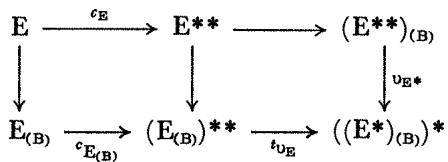
\includegraphics[keepaspectratio]{images/part003_7dd43288.jpg}}

是交换的。

\begin{enumerate}
\def\labelenumi{\arabic{enumi}.}
\setcounter{enumi}{4}
\item
  设 K 为一个域，A 为乘积环 \(K^{N}\) ，a 为 A 的理想 \(K^{(N)}\) ，B 为环 A/a。证明 a 是投射 A-模但不是有限生成的，尽管 \(a_{(B)} = \{0\}\) 。
\item
  设环 A 和 B 如 §1 习题 7 中所定义，令 M 为一个 A-模；证明 M 是有限生成的（相应地，自由的、投射的）当且仅当 \(M \otimes_{A} B\) 是有限生成的（相应地，自由的、投射的）。
\item
  设 \(\rho: A \to B\) 是一个环同态。对每个左 B-模 \(F\) ，定义典范的 B-模同态
\end{enumerate}

\[
\mathbf {F} \rightarrow \tilde {\rho} (\rho_ {*} (\mathbf {F}))
\]

并证明若 E 是一个左 A-模，则复合映射

\[
\begin{array}{r l} & {\tilde {\rho} (\mathbf {E}) \to \tilde {\rho} (\rho_ {*} (\tilde {\rho} (\mathbf {E}))) \to \tilde {\rho} (\mathbf {E})} \\ & {\rho_ {*} (\mathbf {F}) \to \rho_ {*} (\tilde {\rho} (\rho_ {*} (\mathbf {F}))) \to \rho_ {*} (\mathbf {F})} \end{array}
\]

是恒等映射。

\BourbakiExercisesSection

\begin{enumerate}
\def\labelenumi{\arabic{enumi}.}
\item
  设 \((\mathbf{E}_n, f_{nm})\) 是 \(\mathbf{Z}\) -模的逆向系统，其指标集为 \(\mathbf{N}\) ，使得 \(\mathbf{E}_n = \mathbf{Z}\) （对于所有 \(n\) ），并且对于 \(n \leqslant m\) ， \(f_{nm}\) 是映射 \(x \mapsto 3^{m - n}x\) 。对所有 \(n\) ，设 \(u_n\) 为典范映射 \(\mathbf{E}_n \to \mathbf{Z}/2\mathbf{Z}\) 。证明 \((u_n)\) 是由满射线性映射组成的逆向系统，但 \(\lim u_n\) 不是满射。
\item
  设 \((\mathbf{E}_{\alpha}, f_{\beta\alpha})\) 是 A-模的一个正向系统。证明 A-模 \(\lim_{\rightarrow} E_{\alpha}\) 典范同构于直和 \(\bigoplus_{\alpha} E_{\alpha} = F\) 关于子模 N 的商模，N 由形如 \(j_{\beta}(f_{\beta\alpha}(x_{\alpha})) - j_{\alpha}(x_{\alpha})\) 的元素生成（对于每个有序对 \((\alpha, \beta)\) （满足 \(\alpha \leqslant \beta\) ）以及所有 \(x_{\alpha} \in E_{\alpha}\) ），其中诸 \(j_{\alpha}: E_{\alpha} \to F\) 是典范单射。
\item
  设 \((\mathbf{F}_n, f_{mn})\) 为 \(\mathbf{Z}\) -模的正向系统，使得 \(\mathbf{F}_n\) 等于 \(\mathbf{U}_p\) （ \(\S 1\) ，习题 12(d)）对所有 \(n \geqslant 0\) ，并且 \(f_{mn}\) 是自同态 \(x \mapsto p^{m-n}x\) （ \(\mathbf{U}_p\) 的）（对于 \(n \leqslant m\) ）。证明 \(\lim_{\longrightarrow} \mathbf{F}_n = \{0\}\) ，尽管诸 \(f_{mn}\) 是满射。
\item
  设 \((\mathbf{F}_{\alpha}, f_{\beta \alpha})\) 是 A-模的一个正向系统。
\end{enumerate}

\begin{enumerate}
\def\labelenumi{(\alph{enumi})}
\tightlist
\item
  对每个 A-模 E，定义一个典范 Z-模同态
\end{enumerate}

\[
\varepsilon : \varinjlim \operatorname{Hom} _ {\mathbf {A}} (\mathrm{E}, \mathrm{F} _ {\alpha}) \rightarrow \operatorname{Hom} _ {\mathbf {A}} (\mathrm{E}, \varinjlim \mathrm{F} _ {\alpha}).
\]

\begin{enumerate}
\def\labelenumi{(\alph{enumi})}
\setcounter{enumi}{1}
\item
  证明：若 E 是有限生成的，则 \(\varepsilon\) 是单射。给出一个例子，其中 \(\varepsilon\) 不是单射（参见习题 3，取 \(E = \lim F_{\alpha}\) ）。
\item
  证明若 E 是有限生成的且诸 \(f_{\beta\alpha}\) 都是单射，则 \(\varepsilon\) 是满射。给出一个例子，其中 \(E = \lim_{\longrightarrow} F_{\alpha}\) 是自由的，诸 \(f_{\beta\alpha}\) 是单射，并且 \(\varepsilon\) 不是满射。
\item
  证明：如果 \(\mathbf{E}\) 是投射的且有限生成的， \(\varepsilon\) 是双射。
\end{enumerate}

\(^{*}(e)\) 设 A 是一个整环，a 是 A 的一个非有限生成的理想。若 \((a_{\alpha})\) 是包含在 a 中的有限生成理想的族，证明 E = A/a 典范同构于诸 \(F_{\alpha} = A/a_{\alpha}\) 的正向极限，但同态 \(\varepsilon\) 不是满射。*
